\section{Berechnung einer Kugel}
Damit später eine Textur für die Sonne erstellt werden kann, muss zuerst eine
Oberfläche generiert werden, die diese Textur aufnehmen kann. Hierfür existieren
verschiedenste Möglichkeiten. Im Falle der Sonne betrachten wir das Modell einer
Kugel, die später manipuliert werden soll, um visuelle Effekte auf ihr
abzubilden. Beim Betrachten der folgenden Algorithmen zur Erzeugung von
Kugeloberflächen wird klar, dass nicht alle Methoden für dieses Vorhaben
geeignet sind. Aus diesem Grund werden die einzelnen Verfahren näher erläutert
und anschließend abgewogen, welcher Algorithmus zur Erzeugung einer
Sonnenoberfläche verwendet werden sollte.

\begin{figure}
  
\includegraphics[width=\columnwidth]{spheres}
  \caption{Vergleich der verschiedenen Resultate der Algorithmen zum Erzeugen von Punkten auf einer Kugel. Links: Fibonacci-Gitter, Mitte: Icosphere, Rechts: Längen-Breitengrad-Gitter.}
  \Description[Darstellung Algorithmen]{Darstellung der Algorithmen zum Erzeugen von Punkten auf Kugeln}
\end{figure}

\subsection{Längengrad-Breitengrad-Gitter}
Die einfachste Möglichkeit, eine Kugeloberfläche zu erzeugen, ist die Verwendung
von Segmentlinien. Im Grunde unterteilt man die gesamte Kugel in Schichten,
deren Umfang schließlich die Oberfläche der Kugel darstellen. Die Mesh-Punkte
(\textit{Vertices}) dieser Schichten, welche als einfache Kreise wahrgenommen
werden können, werden mithilfe von Längen- und Breitengradinformationen
erstellt. Das Resultat ist eine Kugeloberfläche mit erkennbaren Polen an der
Ober- und Unterseite der Oberfläche. Diese entstehen dadurch, dass auch am Rand
der Kugel die gleiche Anzahl an Kanten vorhanden ist, wie am Äquator. Diese
Schichten sind dementsprechend lediglich herunterskaliert und in einem immer
kürzer werdenden Abstand aufeinander geschichtet und Erzeugen eine Überabtastung
am oberen und unteren Rand der Kugel \cite{Gonzalez2009}.

Die Überabtastung an den Polen bzw. die Unterabtastung am Äquator bringt viele
Probleme mit sich. Vor allem, wenn die Oberfläche animiert werden soll,
erscheint die Animation als sehr unregelmäßig. Hierauf wird jedoch in einem
späteren Abschnitt eingegangen, wenn die hier vorgestellten Methoden miteinander
verglichen werden.

\subsection{Fibonacci-Gitter}
Um das Problem der Inhomogenität von Längengrad-Breitengrad-Gittern zu lösen,
können Fibonacci-Gitter verwendet werden. Hierbei werden die Punkte des Gitters
entlang einer Spirale, die sogenannte Fibonacci-Spirale, angeordnet. Wichtig bei
der Konstruktion sind die \textit{Golden-Ratio} $\Phi$ und der
\textit{Golden-Angle} $\alpha$ \cite{Gonzalez2009, Marques2013}.

$$\Phi = \frac{1 + \sqrt{5}}{2} \quad\quad\quad \alpha = 2\pi\left(2 - \Phi\right)$$

Besonders einfach lässt sich bei diesem Algorithmus die Anzahl an Oberflächenpunkte
kontrollieren. Das folgende Beispiel behandelt das Erstellen von $N$ Punkten,
die gleichmäßig verteilt auf der Oberfläche einer Kugel liegen. Zuerst werden
die Längen- und Breitengrade der einzelnen Punkte berechnet.

$$lat_i = arcsin\left(\frac{2i}{N + 1} - 1\right) \quad\quad\quad
lon_i = \alpha \cdot i$$

Anschließend können die räumlichen Koordinaten als Positionsvektor $\vec{p} \in
\mathbb{R}^3$ wie folgt berechnet werden.

\[
\vec{p} =
\left(\begin{array}{c}
    \cos\left(lon\right) cos\left(lat\right) \\
    \sin\left(lon\right) sin\left(lat\right) \\
    \sin\left(lat\right)
\end{array}\right)
\]

Wie man sieht, ist die Erzeugung von homogen verteilten Oberflächenpunkten einer
Kugel mithilfe von Fibonacci-Gittern ziemlich schnell implementiert. Nachteil
dieser Lösung ist, dass lediglich die Punkte bzw. Vertices eines Meshes erzeugt
werden. Um Flächen darstellen zu können, muss nachträglich eine Triangulation
stattfinden. 

\subsection{Icosphere}
Genau wie das Fibonacci-Gitter erzeugt ein Ikosaeder gleichmäßig verteilte
Punkte auf der Oberfläche einer Kugel. Das Verfahren ist trotzdem komplett
unterschiedlich. Anstatt die Vertices des Meshes zu berechnen und
anschließend diese miteinander in Dreiecke zu verbinden, wird eine initiale
Geometry erzeugt, dessen Flächen wiederum in weitere Flächen unterteilt wird.
Dieses Vorgehen wird beliebige Male wiederholt, um eine immer glattere
Oberfläche zu erzeugen. Das Problem bei diesem Algorithmus ist, dass durch
die Unterteilung der Flächen in weitere, kleinere Flächen auf den ersten
Blick nicht abgeschätzt werden kann, wie viele Vertices genau berechnet
werden müssen. Tabelle \ref{table:icosahedron-complexity} zeigt den Anstieg
der benötigten Punkte, die durch $N$ wiederholten Unterteilungsschritten
berechnet werden müssen \cite{Marc2019}. Anhand der Anzahl an Dreiecken fällt ein
exponentielles Wachstum auf, weshalb eine Erhöhung der
Unterteilungsiterationen mit Bedacht durchgeführt werden sollte. Eine kleine
Veränderung von $N$ hat große Auswirkung auf die benötigte Rechenleistung für
das Kugelmesh \cite{BlenderPrimitives}.

\begin{table}
  \caption{Vergleich zwischen Anzahl der Unterteilungsiterationen $N$ und den erzeugten neuen Flächen bzw. Vertices.}
  \label{table:icosahedron-complexity}
  \begin{tabularx}{\columnwidth}{lXX}
    \textbf{N} & \textbf{Anzahl Vertices} & \textbf{Anzahl Dreiecke} \\
    \hline
    1 & 12   & 60 \\
    2 & 42   & 240 \\
    3 & 162  & 960 \\
    4 & 642  & 3840 \\
    5 & 2562 & 15360
  \end{tabularx}
\end{table}

\subsection{Wahl eines Algorithmus' für die Sonne}
Da in den voherigen Abschnitten einige Algorithmen zum Erzeugen von Punkten
auf einer Kugeloberfläche besprochen wurden, muss nun ein geeigneter
Algorithmus ausgewählt werden, welcher zur Beschaffenheit der Sonne passt.
Außerdem muss berücksichtigt werden, dass die Oberfläche in späteren
Schritten manipuliert und animiert werden soll. Dabei ist es wichtig zu
berücksichtigen, dass sich die Oberfläche der Sonne überall gleichmäßig
verhalten soll. Aus diesem Grund kann das Längengrad-Breitengrad-Gitter nicht
verwendet werden. Das Problem mit diesem Gitter ist, dass es eine
Überabtastung an den Polen bzw. eine Unterabtastung am Äquator besitzt. Eine
Oberflächenbewegung wäre daher sehr unregelmäßig und entspricht auch nicht dem
originalen Vorbild.

Eine elegantere Lösung wäre die Verwendung des Fibonacci-Gitters. Die Anzahl
der Punkte sind frei wählbar und werden homogen auf der Oberfläche verteilt.
Auch ist die Berechnung der Positionen nicht komplex. Jedoch stößt man auf
Probleme beim erstellen der Flächen basierend auf den Punkten wie in
Abbildung \ref{fig:fibo-lattice-hole} zu sehen. Das Problem liegt beim
Verbinden der letzten Vertices im Mesh, welche nach einer
Delaunay-Triangulation ein Loch hervorrufen. Die Herausforderung ist, dieses
Loch genau so homogen zu schließen, wie den Rest der Oberfläche
\cite{RedBlobGames}.

\begin{figure}
  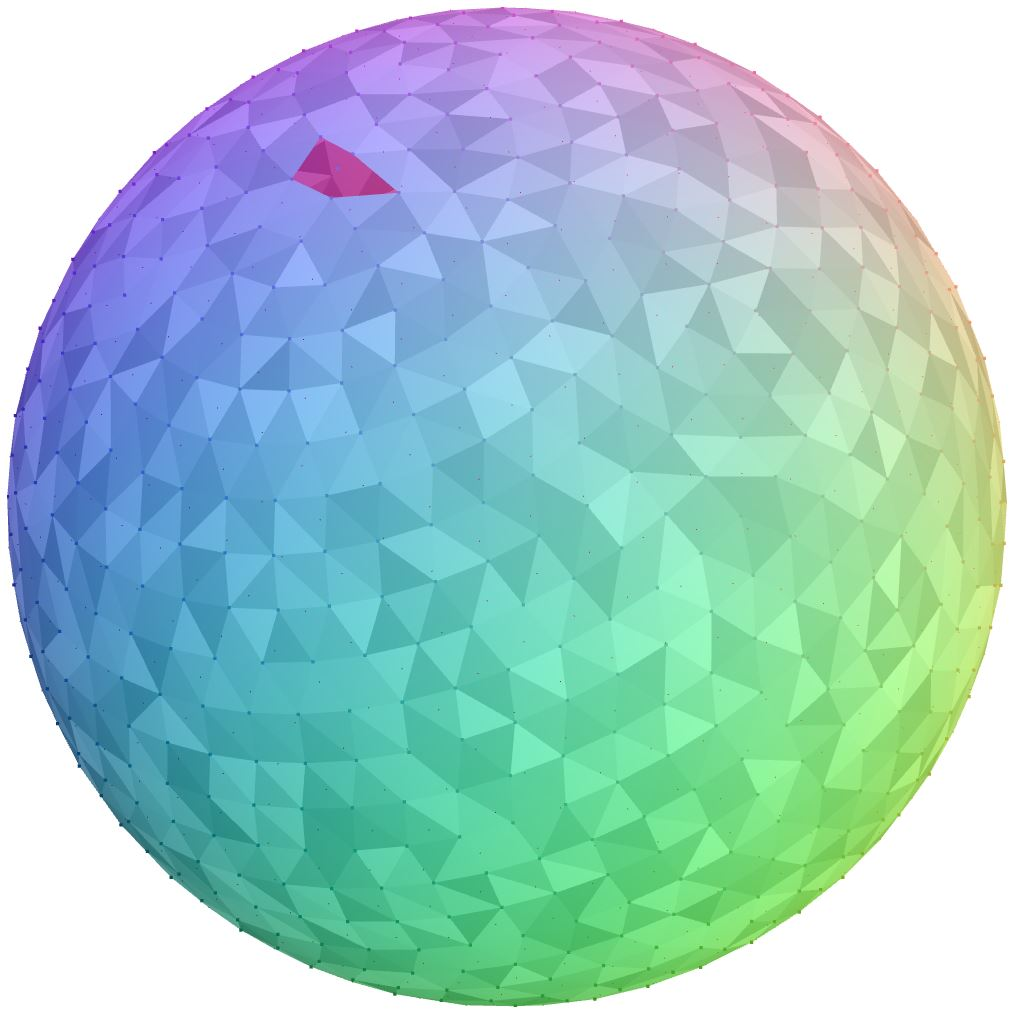
\includegraphics[width=0.6\columnwidth]{fibonacci-sphere-hole}
  \caption{Loch nach dem Ausführen einer Delaunay-Triangulation auf einem Fibonacci-Gitter.}
  \Description[Fibonacci-Gitter-Loch]{Das Loch nach dem Ausführen einer Delaunay-Triangulation auf ein Fibonacci-Gitter}
  \label{fig:fibo-lattice-hole}
\end{figure}

Die wohl am besten geeignete Lösung für das Erzeugen einer Sonnenoberfläche
ist daher die \textit{Icosphere}. Auch, wenn die Anzahl der Punkte bzw. Dreiecke
des Meshes nach jeder neuen Unterteilungsiteration drastisch ansteigen, kann bereits
nach wenigen Iterationen eine erkennbare Kugel mit gleichverteilten Eckpunkten erzeugt
werden. Auch ist die Geometrie geschlossen.